\section{NAT and Link Layer}
\subsection{Obtaining Host IP Addresses -- DHCP}
\begin{itemize}
    \item Networks are free to assign addresses within block to hosts
    \item Tedious and error-prone, e.g. laptop moving between buildings
    \item Solution: Dynamic Host Configuration Protocol
          \begin{itemize}
              \item Client: DHCP Discover to 255.255.255.255 (broadcast)
              \item Server(s): DHCP Offer to 255.255.255.255
              \item Client: choose offer, DHCP Request
              \item DHCP ACK
          \end{itemize}
    \item Result: address, gateway, netmask, DNS Server
\end{itemize}

\subsection{We're running out of internet addresses}
\begin{tcolorbox}[colframe=red!40!white,colback=yellow!20,title=We're running out of internet addresses]
    Don't panic, but we're running out of internet addresses.

    Not domain names -- those website names that you see at the top of this page and which always start with some semblance of ``http://'' and ``www.''

    We've got plenty of those.

    But, according to statements from prominent internet thinkers this week, we may run out of internet protocol -- or IP -- addresses in less than a year.

    IP addresses are numbers assigned to all of the devices -- computers, phones, cars, wireless sensors, etc. -- that log on to the internet.

    According to the blog ReadWriteWeb, the internet is changing and evolving so quickly -- with so many new types of devices connecting -- that we're running out of numbers to assign to all of these Web-enabled electronics.

    \url{https://www.cnn.com/2010/TECH/innovation/07/23/internet.addresses/index.html}
\end{tcolorbox}
\subsection{The internet has (kind of) run out of space}
\begin{tcolorbox}[colframe=red!40!white,colback=yellow!20,title=The internet has (kind of) run out of space]
    On Thursday, the internet as we know it ran out of space.

    The nonprofit group that assigns addresses to service providers announced that, on Thursday morning, it allocated the last free internet addresses available from the current pool used for most of the internet's history.

    ``This is an historic day in the history of the internet, and one we have been anticipating for quite some time,'' said Raul Echeberria, chairman of the Number Resource Organization.

    But fear not. The group has seen this coming for more than a decade and is ready with a new pool of addresses that it expects to last, well, forever.

    John Curran, CEO of the American Registry for Internet Numbers, said the old pool of Internet Protocol addresses had about 4.3 billion addresses.

    ``A billion sounds like a lot,'' Curran said Thursday morning. ``But when you think that there's nearly 7 billion people on the planet, and you're talking about two, three, four, five addresses per person (for some Web users), obviously 4.3 billion isn't enough.''

    \url{http://edition.cnn.com/2011/TECH/web/02/03/internet.addresses.gone/index.html}
\end{tcolorbox}

\subsection{The Last 5 Allocations}
\begin{verbatim}
102/8    AfriNIC     2011-02    whois.afrinic.net   ALLOCATED!
103/8    APNIC       2011-02    whois.apnic.net     ALLOCATED!
104/8    ARIN        2011-02    whois.arin.net      ALLOCATED!
179/8    LACNIC      2011-02    whois.lacnic.net    ALLOCATED!
185/8    RIPE NCC    2011-02    whois.ripe.net      ALLOCATED!
\end{verbatim}
\begin{itemize}
    \item IP addresses: $2^32$ is only $4$ billion
    \item How do we connect devices if we run out of IP addresses?
          \begin{itemize}
              \item IPv6
              \item Other solutions?
          \end{itemize}
\end{itemize}

\subsection{Port-Translating NAT}
\begin{itemize}
    \item Two hosts communicate with the same destination
          \begin{itemize}
              \item Destination needs to differentiate between the two
          \end{itemize}
    \item Map outgoing packets
          \begin{itemize}
              \item Change source address and source port
          \end{itemize}
    \item Maintain a translation table
          \begin{itemize}
              \item Map of $(\texttt{src addr}, \texttt{port \#})$ to $(\texttt{NAT addr}, \texttt{new port \#})$
          \end{itemize}
    \item Map incoming packets
          \begin{itemize}
              \item Map the destination address/port to the local host
          \end{itemize}
\end{itemize}

\subsection{Network Address Translation Example}
\begin{figure}[H]
    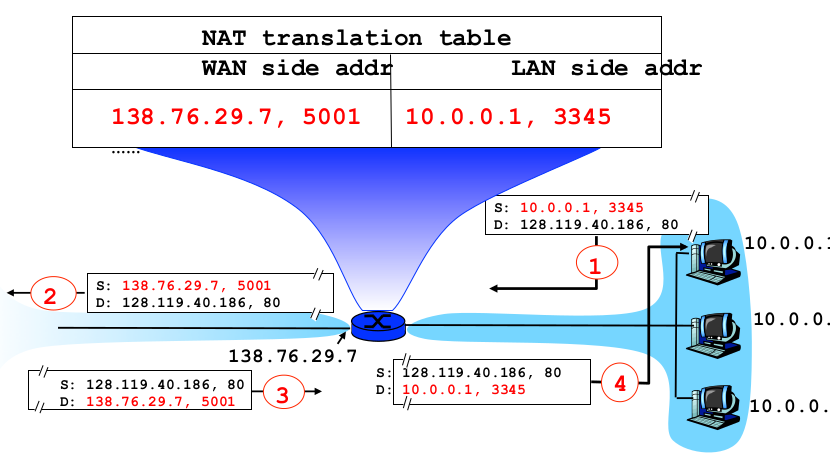
\includegraphics[scale=0.5]{lazy/network-address-translation.png}
\end{figure}

\subsection{Maintaining the Mapping Table}
\begin{itemize}
    \item Create an entry upon seeing an outgoing packet
          \begin{itemize}
              \item Packet with new $(\texttt{src addr}, \texttt{src port})$ pair
          \end{itemize}
    \item Eventually, need to delete entries to free up \#'s
          \begin{itemize}
              \item When? If not pockets arrive before a timeout
              \item (At risk of disrupting a temporarily idle connection)
          \end{itemize}
    \item An example of \emph{soft state}
          \begin{itemize}
              \item i.e., removing state if not refreshed for a while
          \end{itemize}
\end{itemize}

\subsection{P2P Connections across NAT}
\begin{figure}[H]
    \tikzsetnextfilename{p2p-across-nats}
    \begin{tikzpicture}[every node/.style={draw=blue,fill=blue!40!white}]
        \node[label=below:{192.168.1.100},circle] (c1) {C1};
        \node[label=below:{129.7.240.2},rectangle,minimum height=2cm,right=of c1] (nat1) {NAT1};
        \node[circle,above right=0.25cm and 1cm of nat1] (relay) {Relay};
        \node[label=below:{128.125.124.3},rectangle,minimum height=2cm,below right=0.25cm and 1 cm of relay] (nat2) {NAT2};
        \node[label=below:{192.168.1.100},circle,right=of nat2] (c2) {C2};
    \end{tikzpicture}
\end{figure}

\subsection{NAT Traversal}
\begin{itemize}
    \item How do we connect to ``servers'' behind a NAT?
\end{itemize}
\url{https://en.wikipedia.org/wiki/NAT_traversal}

\subsection{IPv6}
\begin{itemize}
    \item Address space 128 bits
    \item Other features
          \begin{itemize}
              \item Multicast
              \item Stateless addressing
          \end{itemize}
\end{itemize}

\subsection{IPv6 Adoption}
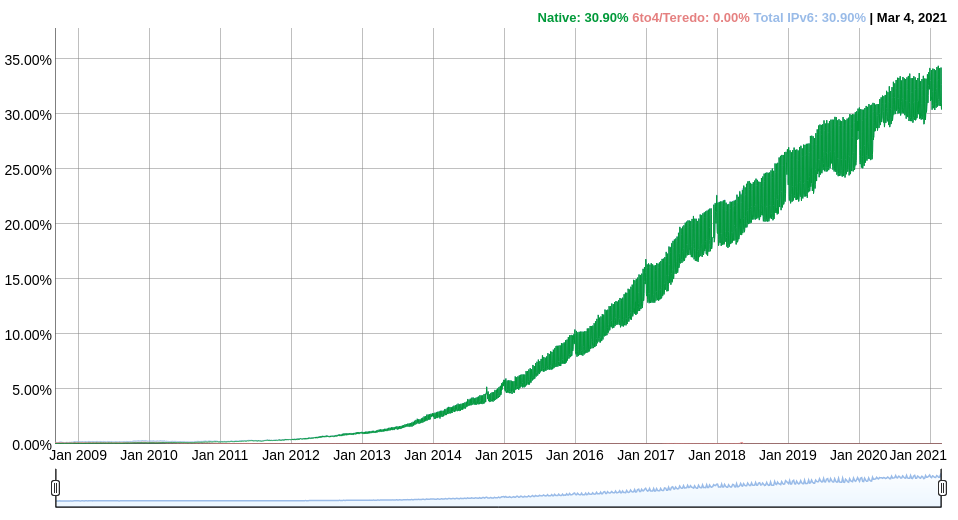
\includegraphics[scale=0.5]{lazy/ipv6adoption.png}

\subsection{Link Layer}
\begin{itemize}
    \item Error Detection
    \item Reliability
    \item Media Access
    \item Ethernet
\end{itemize}

\subsection{Error Detection}
\begin{itemize}
    \item Idea: add redundant information to catch errors in packet
    \item Used in multiple layers
    \item Three examples:
          \begin{itemize}
              \item Parity
              \item Internet Checksum
              \item CRC
          \end{itemize}
\end{itemize}

\subsection{Simplest Schemes}
\begin{itemize}
    \item Repeat Frame
          \begin{itemize}
              \item High overhead
              \item Can't correct error
          \end{itemize}
    \item Parity
          \begin{itemize}
              \item Can detect odd number of bit errors
              \item No correction
          \end{itemize}
\end{itemize}

\subsection{Reliable Delivery}
\begin{itemize}
    \item Error detection can discard bad packets
    \item Problem: if bad packets are lost, how can we ensure reliable delivery?
          \begin{itemize}[nosep]
              \item Exactly-once semantics = at least once + at most once
          \end{itemize}
\end{itemize}
\subsection{At Least Once Semantics}
\begin{itemize}[nosep]
    \item How can the sender know the packet arrived \emph{at least once}?
          \begin{itemize}[nosep]
              \item Acknowledgements + Timeout
          \end{itemize}
    \item Stop and Wait Protocol
          \begin{itemize}[nosep]
              \item S: Sent packet, wait
              \item R: Receive packet, send ACK
              \item S: Receive ACK, send next packet
              \item S: No ACK, timeout and retransmit
          \end{itemize}
\end{itemize}

\subsection{Stop and Wait Problems}
\begin{itemize}[nosep]
    \item Duplicate Data
    \item Duplicate ACKs
    \item Can't fill pipe (remember bandwidth-delay product)
    \item Difficult to set the timeout value
\end{itemize}